% Clean CV/Resume Template, by Bennet B <dev@bennet.cc>
% CC0, Public-Domain
% 
% Permission is hereby granted, free of charge, to any person obtaining a copy
% of this template and associated files (the "Template"), to deal
% in the Template without restriction, including without limitation the rights
% to use, copy, modify, merge, publish, distribute, sublicense, and/or sell
% copies of the Template, and to permit persons to whom the Template is
% furnished to do so, subject to the following conditions:
%
% The above copyright notice and this permission notice shall be included in all
% copies or substantial portions of the Template.
%
% THE TEMPLATE IS PROVIDED "AS IS", WITHOUT WARRANTY OF ANY KIND, EXPRESS OR
% IMPLIED, INCLUDING BUT NOT LIMITED TO THE WARRANTIES OF MERCHANTABILITY,
% FITNESS FOR A PARTICULAR PURPOSE AND NONINFRINGEMENT. IN NO EVENT SHALL THE
% AUTHORS OR COPYRIGHT HOLDERS BE LIABLE FOR ANY CLAIM, DAMAGES OR OTHER
% LIABILITY, WHETHER IN AN ACTION OF CONTRACT, TORT OR OTHERWISE, ARISING FROM,
% OUT OF OR IN CONNECTION WITH THE TEMPLATE OR THE USE OR OTHER DEALINGS IN THE
% TEMPLATE.
%
% based on Modern CV by Habib Semouma
% https://www.overleaf.com/latex/templates/modern-cv-slash-resume-template/vjrqdkpjckwj
%
% 
\documentclass[oneside]{article}

\usepackage{wallpaper}
\usepackage{geometry}
\usepackage[
    unicode=true,
    bookmarks=true,
    bookmarksnumbered=false,
    bookmarksopen=true,
    bookmarksopenlevel=1,
    breaklinks=false,
    pdfborder={0 0 0},
    backref=false,
    colorlinks=false
    ]{hyperref}
\usepackage{lastpage}
\usepackage{hyphenat}
\usepackage{hyphsubst}
\usepackage{tabularx}
\usepackage{moresize}
\usepackage[document]{ragged2e}
% \usepackage{parskip}

\usepackage[scaled]{helvet}
\usepackage{fontawesome5}
\usepackage[defaultfam,tabular,oldstyle]{montserrat}
\usepackage[T1]{fontenc}
\renewcommand*\oldstylenums[1]{{\fontfamily{Montserrat-TOsF}\selectfont #1}}

\usepackage{titlesec}
\usepackage{xcolor}
\usepackage{tikz}

\setlength{\parindent}{0pt}
\titleformat{\section}{\normalfont}{}{0pt}{}

\renewcommand{\arraystretch}{1.4}

\setlength\fboxrule{0pt}
\setlength\fboxsep{12pt}
% \setlength{\parskip}{.5\baselineskip plus 2pt}
% \renewcommand{\baselinestretch}{1.1}

\titlespacing{\section}{0pt}{1.5ex plus .1ex minus .2ex}{1pc}

\newcolumntype{Y}{>{\RaggedRight\arraybackslash}X}

% Change PDF Meta Info here
\hypersetup{
    pdftitle={John Doe - CV - English},
    pdfauthor={John Doe},
    pdfsubject={CV}
}

% Paper size
\geometry{
    a4paper,
    left=0pt,
    right=0pt,
    top=0pt,
    bottom=0pt,
    nohead,
    % includefoot,
    nomarginpar
}

% Background Color of the Sidebar Column
\definecolor{sidebg}{cmyk}{1, 0.02, 0, 0.56}
% Background Color of the Main Column
\definecolor{mainbg}{cmyk}{0, 0, 0.07, 0.04}

% Text Color of the Main Column
\definecolor{maintext}{cmyk}{1, 0.02, 0, 0.8}
% Text Color of the Sidebar Column
\definecolor{sidetext}{cmyk}{0, 0, 0.07, 0.04}

\pagecolor{mainbg}

\begin{document}
\setlength{\topskip}{0pt}\setlength{\footskip}{0pt}%
\fcolorbox{red}{sidebg}{%
    \begin{minipage}[t][\textheight-2\fboxsep-2\fboxrule][t]{\dimexpr0.40\textwidth-2\fboxrule-2\fboxsep\relax}
        \color{sidetext}
        %%%%%%%%%%%%%%%%%%%%%%%%%%%%%%%%%%%%%%%%%%%%%%%%%%%%
        % YOUR NAME, PRONOUNS, OCCUPATION(s), AND HEADSHOT
        {\bfseries\scshape\HUGE Huy} \\
        {\bfseries\scshape\Huge Huynh} \qquad {he/him}
        \vspace{.3cm} \\
        Software & Full Stack Development Intern, \\
        Seeking Software & Full Stack Engineer Roles 
        \\
        \begin{center}
            \begin{tikzpicture}
            \clip (0,0) circle (2.5cm) node[anchor=center] {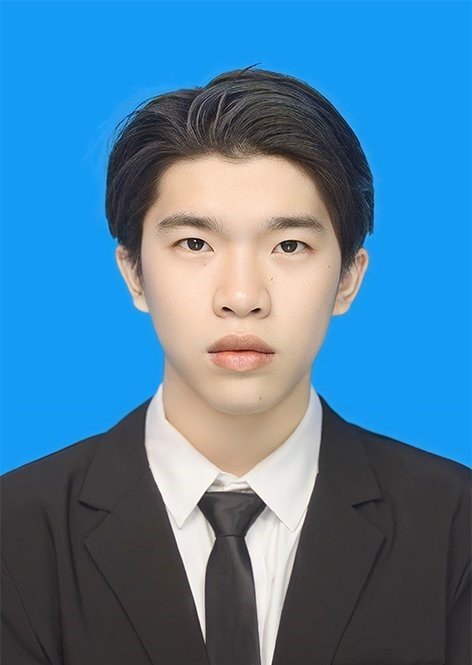
\includegraphics[width=5cm]{huyhuynh01.jpg}}; 
            \end{tikzpicture}
        \end{center}
        \vspace{.3cm}
        %%%%%%%%%%%%%%%%%%%%%%%%%%%%%%%%%%%%%%%%%%%%%%%%%%%%
        % YOUR PERSONAL INFROMATION
        \phantomsection{}
        \addcontentsline{toc}{section}{Personal info}
        \section*{\large Personal info}
        \begin{tabularx}{\textwidth}{cY}
            \faStarOfLife{} & 03/01/2004 \\
            \faPhone{}      & +84-924-202-149 \\
            \faEnvelope{}   & \href{mailto:huykyunh.k@gmail.com}{huykyunh.k@gmail.com} \\
            \faMapMarker{}  & Long Xuyen City, An Giang, Vietnam \\
        \end{tabularx}
        \vspace{.3cm} \\    
        \rule{\linewidth}{0.4pt} \\
        %%%%%%%%%%%%%%%%%%%%%%%%%%%%%%%%%%%%%%%%%%%%%%%%%%%%%%%%%
        % YOUR LINKS, YOU MAY ALSO ADD A PERSONAL WEBSITE OR PORTFOLIO
        \phantomsection{}
        \addcontentsline{toc}{section}{Links}
        \section*{\large Links}
        \begin{tabular}{cl}
        %    \faCode{}     & \href{https://example.com}{example.com}
            \faGithub{}   & \href{https://github.com/hkhuang07}{github.com/hkhuang07} \\
            \faLinkedin{} & \href{https://www.linkedin.com/in/hkhuang07/}{linkedin.com/in/hkhuang07} \\
            \faFacebook{}     & \href{https://https://www.facebook.com/hk.huang07}{facebook.com/hkhuang07} \\
        \end{tabular}
        \vspace{10pt} \\
        \rule{\linewidth}{0.4pt} \\
        %%%%%%%%%%%%%%%%%%%%%%%%%%%%%%%%%%%%%%%%%%%%%%%%%%%%%%%%%%%%
        % LANGUAGES
        \phantomsection
        \addcontentsline{toc}{section}{Languages}
        \section*{\large Languages}
        \begin{tabular}{cl}
            \faLanguage{} & \textbf{Vietnamese:} Native \\
            \faLanguage{} & \textbf{English:} Intermediate (B1) \\
            \faLanguage{} & \textbf{Chinese:} Basic \\
        \end{tabular}
        \vspace{.3cm}
        \\
        \rule{\linewidth}{0.4pt}
        %%%%%%%%%%%%%%%%%%%%%%%%%%%%%%%%%%%%%%%%%%%%%%%%%%%%%%%%%%%%%%%%
        % GITHUB PROFILE
        \phantomsection{}
        \addcontentsline{toc}{section}{GitHub Profile}
        \section*{\large GitHub Profile}
        \begin{tabular}{cl}
            \faGithub{} & \href{https://github.com/hkhuang07}{github.com/hkhuang07} \\
        \end{tabular}
        \vspace{.3cm}
        
        \textbf{Projects:} \\ % Xuống hàng trước "Projects"
        \begin{itemize}
            \setlength{\itemsep}{2pt}
            \item .NET (2 projects),\\Android (1 project),\\ NodeJS (1 project),\\others (6 projects)
           
        \end{itemize}
        \vspace{10pt} \\
        \rule{\linewidth}{0.4pt} \\

        %%%%%%%%%%%%%%%%%%%%%%%%%%%%%%%%%%%%%%%%%%%%%%%%%%%%%%%%%%%%%%%%
        
    \end{minipage}
}
\hfill
\fcolorbox{red}{mainbg}{%
    \begin{minipage}[t][\dimexpr\textheight-2\fboxrule-2\fboxsep\relax][t]{\dimexpr0.6\textwidth-2\fboxrule-2\fboxsep\relax}
        \color{maintext}
        %%%%%%%%%%%%%%%%%%%%%%%%%%%%%%%%%%%%%%%%%%%%%%%%%%%%%%%%%%
        % YOUR SKILLS
        % Add/Remove as seen fit, Icons: https://packages.oth-regensburg.de/ctan/fonts/fontawesome5/doc/fontawesome5.pdf
        \phantomsection{}
        \addcontentsline{toc}{section}{Skills}
        \section*{\scshape\Large Skills \rule{\linewidth}{0.4pt}}
        \vspace{-1.5ex}
        
        {\large \textbf{Programming Languages}}
        \begin{itemize}
            \setlength{\itemsep}{-3pt}
            \item C\#, C, C++, Python, Java, JavaScript, PHP (Intermediate)
            \item Batch Script, Assembly language (Basic)
        \end{itemize}
        
        {\large \textbf{Markup & Styling Languages}}
        \begin{itemize}
            \setlength{\itemsep}{-3pt}
            \item Markdown, HTML, CSS, LaTeX
        \end{itemize}
        
        {\large \textbf{Frameworks \& Libraries}}
        \begin{itemize}
            \setlength{\itemsep}{-3pt}
            \item ASP.NET Core (Entity Framework Core)
            \item Android Jetpack, ReactJS / Next.js, Node.js (Express.js)
            \item Tailwind CSS, Bootstrap 5
        \end{itemize}
        
        {\large \textbf{Technologies \& Platforms}}
        \begin{itemize}
            \setlength{\itemsep}{-3pt}
            \item Supabase, Firebase, MongoDB Atlas
            \item Cloud Computing Concepts (Basic understanding of AWS/GCP/Azure)
            \item Git \& GitHub, RESTful APIs, Docker (Basic)
        \end{itemize}
        
        {\large \textbf{Databases}}
        \begin{itemize}
            \setlength{\itemsep}{-3pt}
            \item SQL Server, MySQL, Oracle (Intermediate)
            \item PostgreSQL, MongoDB, SQLite (Basic)
        \end{itemize}
        
        {\large \textbf{Operating Systems}}
        \begin{itemize}
            \setlength{\itemsep}{-3pt}
            \item Windows, Linux
        \end{itemize}
        
        {\large \textbf{Development Tools}}
        \begin{itemize}
            \setlength{\itemsep}{-3pt}
            \item Visual Studio, Visual Studio Code, Android Studio
            \item PyCharm, IntelliJ IDEA, Eclipse, VMware
        \end{itemize}
        %%%%%%%%%%%%%%%%%%%%%%%%%%%%%%%%%%%%%%%%%%%%%%%%%%%%%%%%%%%
        % EDUCATION
        \phantomsection{}
        \addcontentsline{toc}{section}{Education}
        \section*{\scshape\Large Education \rule{\linewidth}{0.4pt}}
        %
        {\large \textbf{An Giang University}} \\
        {{\fontseries{medium}\selectfont Bachelor of Science in Information Technology}} \\
        {\scshape\fontseries{light}\selectfont\footnotesize An Giang, Vietnam [2022 \textendash{} 2026] (Expected Graduation)}
        \begin{itemize}
            \setlength{\itemsep}{-3pt}
            \item Major in Information Technology
            \item Relevant Coursework:
            \begin{itemize}
                \setlength{\itemsep}{-3pt}
                \item Information Management System Programming, Mobile Device Programming, IoT Programming,       Cloud Computing, Web Programming, PHP Web Technology
                \item Artificial Intelligence, Machine Learning, Data Mining
                \item Network Administrator, Computer Network, Network Communication Programming, Information Security
                \item Computer Architecture, Operating System, Data Structure and Algorithms \item Oracle-SQL Server Database, 
                \item Analyze \& Design Information System and OOP Software
            \end{itemize}
        \end{itemize}
        %%%%%%%%%%%%%%%%%%%%%%%%%%%%%%%%%%%%%%%%%%%%%%%%%%%%%%%%%%%
        % EXPERIENCES
        \phantomsection{}
        \addcontentsline{toc}{section}{Experiences}
        \section*{\scshape\Large Experiences \rule{\linewidth}{0.4pt}}
        %
        {\large \textbf{Massive Open Online Course}} \\
        {{\fontseries{medium}\selectfont edX: CS50: Introduction to Computer Science}} \\
        {\scshape\fontseries{light}\selectfont\footnotesize June - July 2024}
        \begin{itemize}
            \setlength{\itemsep}{-3pt}
            \item Gained a foundational understanding of computer science and programming concepts.
            \item Explored various topics including algorithms, data structures, web development, and database design.
            \item Developed problem-solving skills through hands-on programming assignments in C, Python, SQL, and HTML/CSS/JavaScript.
        \end{itemize}
        \vspace{10pt} \\
        \rule{\linewidth}{0.4pt} \\
            
        
        \vspace{10pt} \\
        \rule{\linewidth}{0.4pt} \\
    
        \vfill%
        {\hfill\small\fontseries{extralight}\selectfont Page \thepage of \pageref{LastPage}\hfill}
        \end{minipage}
}%
\newpage
%%%%%%%%%%%%%%%%%%%%%%%%%%%%%%%%%
% PAGE 2
%%%%%%%%%%%%%%%%%%%%%%%%%%%%%%%%%
\fcolorbox{red}{mainbg}{%
    \begin{minipage}[t][\dimexpr\textheight-2\fboxrule-2\fboxsep\relax][t]{\dimexpr0.6\textwidth-2\fboxrule-2\fboxsep\relax}
        \color{maintext}
        % \vspace{.6cm}
        %%%%%%%%%%%%%%%%%%%%%%%%%%%%%%%%%%%%%%%%%%%%%%%%
        % PROJECTS
        \phantomsection
        \addcontentsline{toc}{section}{Projects}
        \section*{\scshape\Large Projects \rule{\linewidth}{0.4pt}}
        \begin{justify}
        \setlength{\parindent}{0pt}
        {\large \textbf{Sales Management System - Client-Server Model}} \\
        {\scshape\fontseries{light}\selectfont\footnotesize Individual Project \qquad ( July 2025 )} \\
        A sales management application for electronics stores, built on a robust client-server architecture. The system uses an efficient multi-threaded approach to handle concurrent operations and ensures data integrity with a clean 4-Layer architecture( Client-Server-Business Logic-Data Acess). \\[1ex]
        \textbf{Technologies:} C\#, .NET, Entity Framework Core, SQL Server, TCP/IP Sockets, Multi-threading, Newtonsoft.Json, Windows Forms UI, Unit of Work Pattern, DTOs \\
        Repository: \href{https://github.com/hkhuang07/Sales-Management-Client-Server-Model-Socket-Multil-Threads}{github.com/hkhuang07/Sales-Management-Client-Server-Model-Socket-Multil-Threads} \\
        
        {\large \textbf{Sales Management Mobile App \textendash{} Firebase Cloud}} \\
        {\scshape\fontseries{light}\selectfont\footnotesize Individual Project \qquad ( May\textendash{}June 2025 )} \\
        An Android mobile application for sales and product management, offering distinct functionalities for administrators and regular users. The app leverages Firebase for secure authentication and real-time data storage, ensuring a scalable and modern backend solution. \\[1ex]
        \textbf{Technologies:} Java, Android, Google Firebase (Authentication, Cloud Firestore, FCM), AndroidX, Material Design Components \\
        Repository: \href{https://github.com/hkhuang07/Sales-Management-Mobile-App-Firebase}{github.com/hkhuang07/Sales-Management-Mobile-App-Firebase} \\
        
        {\large \textbf{Sales Management Website \textendash{} Supabase Cloud }} \\
        {\scshape\fontseries{light}\selectfont\footnotesize Individual Project \qquad ( March - April 2025 )} \\
        A web-based online marketplace for second-hand products. The project provides an intuitive platform for buying and selling items, with distinct functionalities for guests, users, managers, and administrators. It leverages Supabase as a Backend-as-a-Service (BaaS) for data storage and authentication. \\[1ex]
        \textbf{Technologies:} HTML5, CSS3, JavaScript (ES6+), Bootstrap 5, jQuery, Supabase (Auth, PostgreSQL, Storage) \\
        Repository: \href{https://github.com/hkhuang07/Sales-Management-Website-Supabase}{github.com/hkhuang07/Sales-Management-Website-Supabase} \\
        Website: \href{https://graceful-profiterole-21b706.netlify.app/}{graceful-profiterole-21b706.netlify.app} \\

        {\large \textbf{Online News \textendash{} NodeJS \textendash{} MongoDB Atlat}} \\
        {\scshape\fontseries{light}\selectfont\footnotesize Individual Project \qquad ( February 2025 )} \\
        A robust online news portal for content creation and Browse. The application features dynamic content display, comprehensive category and user management, and a secure administration panel. It is built using Node.js for the backend and MongoDB Atlas for data persistence. \\[1ex]
        \textbf{Technologies:} Node.js, Express.js, MongoDB Atlas, Mongoose, EJS, Bootstrap, Bcryptjs, Express-session \\
        Repository: \href{https://github.com/hkhuang07/Online-News-Site-NodeJS-MongoDB-Atlat}{github.com/hkhuang07/...} \\
        Website: \href{https://online-news-website-nodejs-mongodb-atlat.onrender.com/}{online-news-website-nodejs-mongodb-atlat.onrender.com}\\
        
        {\large \textbf{CPU Visualizer \textendash{} PyQt6}} \\
        {\scshape\fontseries{light}\selectfont\footnotesize Individual Project \qquad ( June 2025 )} \\
        An interactive simulation tool for a simplified 8-bit CPU. The application visualizes core instruction cycle phases (Fetch-Decode-Execute), real-time register and flag changes, and data flow. It serves as an educational resource for understanding fundamental computer architecture. \\[1ex]
        \textbf{Technologies:} Python, PyQt6\\
        Repository: \href{https://github.com/hkhuang07/CPU-Visualizer-Python-PyQt6}{github.com/hkhuang07/CPU-Visualizer-Python-PyQt6}\\
        
        {\large \textbf{There are many other interesting projects on Github}} \\
        For more, please visit my repository at \href{https://github.com/hkhuang07}{[ github.com/hkhuang07 ]}.
        
        \end{justify}
        \vfill%
        {\hfill\small\fontseries{extralight}\selectfont Page \thepage of \pageref{LastPage}\hfill}
    \end{minipage}
}
\hfill%
\fcolorbox{red}{sidebg}{%
    \begin{minipage}[t][\dimexpr\textheight-2\fboxrule-2\fboxsep\relax][t]{\dimexpr0.4\textwidth-2\fboxrule-2\fboxsep\relax}
        \color{sidetext}
        % \vspace{.5cm}
        %%%%%%%%%%%%%%%%%%%%%%%%%%%%%%%%%%%%%%%%%%%%%%%%%%%%%%%%
        % YOUR NAME AND PREFERED PRONOUS AGAIN AS HEADER
        {\bfseries\scshape\HUGE Huy} \\
        {\bfseries\scshape\Huge Huynh} \qquad {he/him}
        \vspace{.3cm} \\
        %%%%%%%%%%%%%%%%%%%%%%%%%%%%%%%%%%%%%%%%%%%%%%%%%%%%%%%%%%%%
        % CERTIFICATES AND AWARDS RECEIVED
        \phantomsection
        \addcontentsline{toc}{section}{Certificates and Prizes}
        \section*{\large Certificates and Prizes}
        \begin{tabularx}{\textwidth}{cY}
            2025 & English VSTEP B1 \\
        \end{tabularx}
        \vspace{.3cm}
        \\
        \rule{\linewidth}{0.4pt}
        \\
        %%%%%%%%%%%%%%%%%%%%%%%%%%%%%%%%%%%%%%%%%%%%
        % HOBBIES
        % Change Icons here https://packages.oth-regensburg.de/ctan/fonts/fontawesome5/doc/fontawesome5.pdf
        \phantomsection
        \addcontentsline{toc}{section}{Hobbies}
        \section*{\large Hobbies}
        \begin{tabularx}{\textwidth}{cY}
            \faCode{} & Programming \\
            \faCoffee{} & Drink Coffee \\
            \faBook{} & Read Books\\
            \faDumbbell{} & Go Gym and Play Sport \\
        \end{tabularx}
        \vspace{.3cm}
        \\
        \rule{\linewidth}{0.4pt}
    \end{minipage}%
}%
\end{document}